\subsubsection{Hidden categories}
Wikipedia's category structure contains lots of hidden categories which are not displayed at the bottom of an article page for the general users, even if the article is placed under the category. These categories are useful for editing since it is an easy way to all mark categories with something in common, for instance mark all categories with references that needs to be checked. 

Hidden categories are concerned with maintenance and administration, hence not relevant for normal users or for our problem. The next step is therefore to remove all the links to hidden categories, which led to the task of finding all hidden categories. On Wikipedia's information page about \emph{Hidden Categories}\cite{wiki:hiddencat} are 15 385 subcategories listed as immidiate subcategories, but many of these categories have links to their own hidden subcategories which also have to be found. The first attempt was to look through all the links from the category \emph{Hidden Categories}, where 15 006 subcategories where found and marked as not relevant. Since this did not give the expected number, another attempt was made by looking at the file \texttt{enwiki-latest-page\_props.sql.gz}, where figure \ref{fig:pageprops} shows how  hidden categories are marked in the table. The next attempt was therefore to find all the ids marked with \emph{hiddencat} and find the corresponding category titles in \texttt{enwiki-latest-page.sql.gz}. This approach led to 15 513 categories. To make sure that all hidden categories where found, a test was made to see if all categories from the first attempt was found in the list created from the second attempt. The results showed that all categories found in the first attempt was also found in the second attempt, and the list of all 15 513 category titles whose links should be disregarded from further results. 

\begin{figure}[h]
\centering
\begin{lstlisting}
(747593,'hiddencat','',NULL)
\end{lstlisting}
\caption[Insert statement for hidden category]{Excerpt from the file \texttt{enwiki-latest-page\_props.sql.gz} where we can see that hidden categories are marked with \emph{hiddencat}}
\label{fig:pageprops}
\end{figure}

The hidden categories have to be removed carefully because they might be subcategories of visible categories or have visible categorise as their own subcategories. An example of this can be seen in figure \ref{fig:stevie_wonder_hidden}, where the double rounded rectangle is a hidden category, the rounded rectangle is a normal (visible) category and the rectangle is the article about \emph{Stevie Wonder}.
%Hidden categories can not be disregard
%19103360 article links, 391482 category links skipped

%An example of such a structure can be found from the categories leading to the article about the singer Stevie Wonder. 

\begin{figure}[h]
\centering
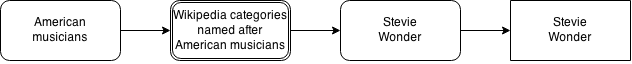
\includegraphics[width=\textwidth]{Chapters/Implementation/HiddenCategories/Stevie_wonder_hidden}
\caption[Example path with hidden category]{An excerpt of one path leading to the article about to Stevie Wonder, where the path contains a hidden category. }
\label{fig:stevie_wonder_hidden}
\end{figure}

The desirable visible paths for all articles are paths without hidden categories. The next step is therefore to change the structure so that hidden categories are removed from the structure, but without loosing any of the subcategories which might contain relevant information or  important links. Example of a how a path can be transformed is figure \ref{fig:stevie_wonder} which is the excerpt from the path in figure \ref{fig:stevie_wonder_hidden} without the hidden categories. 

\begin{figure}[h]
\centering
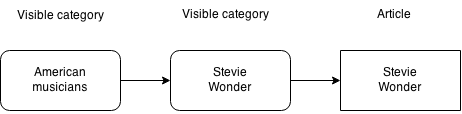
\includegraphics[width=.7\textwidth]{Chapters/Implementation/HiddenCategories/Stevie_wonder}
\caption[Example path without hidden category]{The desirable output of the excerpt of the path leading to the article about Stevie Wonder where the hidden category is removed from the path}
\label{fig:stevie_wonder}
\end{figure}


Table \ref{tab:withouthiddencat} shows how number of links between categories, and between categories and articles are reduced when hidden categories are not considered. 

%The main reason to reduce number of links is to reduce the complexity 

\begin{table}[h]
\centering
\begin{tabular}{l|c|c}
\textbf{Links between...} & \textbf{W/ Hidden Categories} & \textbf{W/o Hidden Categories}  \\ \hline
 \textbf{subcategories} & 1 654 758  & 1 311 275\\
 \textbf{articles and categories} & 4 241 881  & 3 152 873
\end{tabular}
\caption[Number of links without hidden categories]{Number of links removed when all hidden categories are excluded. }
\label{tab:withouthiddencat}
\end{table}
